\documentclass[letterpaper, 10 pt, journal, twoside]{IEEEtran}
\IEEEoverridecommandlockouts
% \input{archive/main.config.tex}
\usepackage{graphicx}
\usepackage{caption}
\usepackage{subcaption}
\usepackage{soul}
\usepackage[dvipsnames]{xcolor}
\hyphenation{op-tical net-works semi-conduc-tor}
\usepackage{xcolor,listings}
\usepackage{textcomp}
\usepackage{todonotes}
\lstset{upquote=true}
\usepackage{array}
% \usepackage{graphicx}
\usepackage{amsmath}
\usepackage{relsize}
\usepackage{amssymb}
\usepackage{color}
\usepackage{threeparttable}
\usepackage{hyperref}

\usepackage{algorithm}
\usepackage{algpseudocode}
% \usepackage[colorlinks,citecolor=blue]{hyperref}

% \usepackage{draftwatermark}

% Packages for drawing
\usepackage{tikz}
\usetikzlibrary{shapes.geometric, arrows,calc}
\tikzstyle{startstop} = [rectangle, rounded corners, minimum width=3cm, minimum height=1cm,text centered, draw=black, fill=none]
\tikzstyle{io} = [trapezium, trapezium left angle=70, trapezium right angle=110, minimum width=3cm, minimum height=1cm, text centered, draw=black, fill=blue!30]
\tikzstyle{process} = [rectangle, minimum width=3.5cm, minimum height=1cm, text centered, draw=black, fill=orange!0]
\tikzstyle{neuron} = [circle, minimum size=3cm, text centered, draw=black, fill=orange!0]
\tikzstyle{decision} = [diamond, minimum width=3cm, minimum height=1cm, text centered, draw=black, fill=green!30]
\tikzstyle{arrow} = [thick,->,>=stealth]

\usepackage{pgfplots}
\pgfplotsset{compat=newest}
\pgfplotsset{plot coordinates/math parser=false}

\usepackage{booktabs}
\usepackage{multirow}

% \usepackage[maxnames=3,firstinits=true,sorting=none,doi=false,url=true,isbn=false]{biblatex}
\usepackage[maxnames=6,firstinits=true,doi=false,url=true,isbn=false]{biblatex}
\addbibresource{dira.bib}


\def \assumptionSGDfirst {1}
\def \assumptionEWCfirst {1}
\def \assumptionEWCsecond {2}

\DeclareMathOperator*{\minimize}{min\text{ }}

\pagenumbering{arabic}


%-------------------------------------------------------------------------------

\begin{document}

% ***************************************************
%  TITLE
% ***************************************************
\title{\textbf{DIRA}: \textbf{D}ynamic Domain \textbf{I}ncremental \textbf{R}egularised \textbf{A}daptation}

\author{Abanoub Ghobrial, Xuan Zheng, Darryl Hond, Hamid Asgari, Kerstin Eder 
\thanks{{\footnotesize
Manuscript  
received ...;
revised ...;  
accepted.... 
Date of publication ...;
date of current version ....

% This research has in part been funded by the ROBOPILOT and CAPRI projects. Both projects are part-funded by the Centre for Connected and Autonomous Vehicles (CCAV), delivered in partnership with Innovate UK under grant numbers 103703 (CAPRI) and 103288 (ROBOPILOT). This research was also supported in part by the UKRI Trustworthy Autonomous Systems Node in Functionality under grant number EP/V026518/1. Also special thanks to S\'everin Lemaignan.

% The Associate Editor for this paper was ....

Abanoub Ghobrial (e-mail: abanoub.ghobrial@bristol.ac.uk), 
Xuan Zheng (e-mail: dq18619@bristol.ac.uk), 
and 
Kerstin Eder (e-mail: kerstin.eder@bristol.ac.uk) 
are with the Trustworthy Systems Lab, Department of Computer Science, University of Bristol, Merchant Ventures Building, Woodland Road, Bristol, BS8 1UB, United Kingdom. 

Darryl Hond (e-mail: darryl.hond@uk.thalesgroup.com),
and
Hamid Asgari (e-mail: hamid.asgari@uk.thalesgroup.com) 
are with Technology and Innovation Research,Thales, Reading, United Kingdom. 

Digital Object Identifier ....
}}}
% \affil{Trustworthy Systems Laboratory, University of Bristol, Bristol, UK}
% \affil{University of West of England, Bristol, UK}
% \affil{Bristol Robotics Laboratory, Bristol, UK}
%
\markboth{IEEE TRANSACTIONS ON Neural Networks and Learning Systems VOL. ..., NO. ..., date...}{Ghobrial \MakeLowercase{\textit{et al.}}: DIRA: Dynamic Domain Incremental Regularised Adaptation}
%
\maketitle

% ***************************************************
%  Abstract
% ***************************************************
\begin{abstract}
\noindent 
Autonomous systems (AS) often use Deep Neural Network (DNN) classifiers to allow them to operate in complex, high-dimensional, non-linear, and dynamically changing environments.
%
Due to the complexity of these environments, DNN classifiers may output misclassifications during operation when they face domains not identified during development.
%
Removing a system from operation for retraining becomes impractical as the number of such AS increases. 
%
To increase AS reliability and overcome this limitation, DNN classifiers need to have the ability to adapt during operation when faced with different operational domains using a few samples (e.g. 100 samples).
%
However, retraining DNNs on a few samples is known to cause catastrophic forgetting. 
%
In this paper, we introduce Dynamic Incremental Regularised Adaptation (DIRA), a framework for operational domain adaption of DNN classifiers using regularisation techniques to overcome catastrophic forgetting and achieve adaptation when retraining using a few samples of the target domain. 
%
Our approach shows improvements on different image classification benchmarks aimed at evaluating robustness to distribution shifts (e.g.CIFAR-10C/100C, ImageNet-C), and produces state-of-the-art performance in comparison with other frameworks from the literature.  
\end{abstract}

\begin{IEEEkeywords}
Adaptation, Machine Learning, Regularisation,  Classifiers, Autonomous Systems
\end{IEEEkeywords}
\IEEEpeerreviewmaketitle 


% ***************************************************
%  Main Body
% ***************************************************
\section{Introduction}
Autonomous systems (AS) often are developed using deep neural network (DNN) classifiers to interact and adapt in dynamically changing real-world environments to achieve their intended goals. 
%
The benefit of using DNNs in autonomous systems is their ability to learn complicated patterns 
% in high-dimensional data 
from complex environments, and thus produce highly non-linear decision boundaries to cope with the complexity of operational environments.
%
However, it is a challenge to verify the behaviour of DNNs.   
%
A popular example of such ASs is self-driving cars. Current research shows that for each self-driving car, an impractical amount of testing is required to verify the system for deployment~\cite{RR-1478-RC}. Innovative methods of increasing the efficiency of testing and validation are actively being developed to make the process more practical, e.g.~\cite{chance2020agency,eder2021complete}. 
%
However, due to the vast operational environments and the enormous effort required in testing to achieve deployment, the community is additionally incorporating trustworthiness assessment of AS to allow for reliable deployment and progressive improvements during the operational lifetime of such systems~\cite{chance2023assessing}. 
%
This follows a two-stage approach presented by Koopman~et.al.~\cite{Koopman2020}, which stipulates that, given an AS passes some minimum safety validation case, the system is deployed and is improved during operation to increase its reliability over time. 
%
Thus, the system is allowed to adapt to dynamically changing operational environments.

The process of continual learning or adaptation can be broken into three stages 1) detection of change in the operational domain, e.g.~\cite{Hond2020,Schaffer2017, Mandelbaum2017, Xing2019}, 2) supply of labels from an oracle or ground truth for new operational domain samples, e.g.~\cite{Barr2015,Zhang2020}, 3) retraining. 
%
Alternatively, 2) and 3) can be substituted by one stage of self-supervised or unsupervised retraining. We aim to investigate this option in future work.
%
In this paper, we focus on point 3), i.e. retraining.

DNN classifiers use gradient-based optimisation algorithms to learn. 
%
The gradient optimiser modifies the decision boundary based on the samples used in training. 
%
Retraining using few samples can result in a phenomenon known as \textit{catastrophic forgetting}, where the model overfits to the few training samples used and does not generalise to the domain distribution~\cite{Goodfellow2014}. 
%
Generally, to overcome catastrophic forgetting, new samples are added to the initial training dataset and the classifier is fully retrained. 
%
Full retraining, however, can be cumbersome to perform during operation. 
% 
%
In this paper, we propose Dynamic Incremental Regularised Adaptation (DIRA), a framework to achieve operational domain adaption by retraining using only few samples from the target domain. 
%
We utilise a combination of regularisation techniques and a retraining scoring approach in our framework to overcome the need for full retraining.

Practically, upon adaptation of AS, reassessment of the system's safety may be required.  
%
The safety compliance of evolving DNN classifiers during operation against a set of requirements or regulations is beyond the scope of this paper, but may be achieved through the use of runtime safety behavioural checkers as presented by Harper~et.al.~\cite{harper2021safety} or by using online methods for quantifying trustworthiness in predictions during operation as shown by Ghobrial et al~\cite{ghobrial2023trustworthiness}. 

In the next section, we discuss related work material. Section~\ref{sec:method} introduces our method.
%
Experimentation Setup and Results \& Discussion are handled by sections~\ref{sec:experimentation} and \ref{sec:results}, respectively.
%
We conclude and discuss future works in Section~\ref{sec:conclusions}.



\section{Related work}
\subsection{Types of Incremental Learning}
Gradually assimilating new information from a continuously changing data stream, known as `continual learning', poses a challenge for deep neural networks. 
%
Continual learning, however, is a fundamental aspect of evolving autonomous systems.
%
In a continual learning setting the problem is broken down into several parts that need to be learned sequentially.
%
In the continual learning literature, these parts are often called \textit{tasks}. Thus, the term tends to have several meanings. 
%
These several connotations of the term task make it difficult to study the different challenges associated with continual learning. 
%
To overcome this problem, Ven et al.\cite{Ven2022}, proposed to brake down continual learning into three incremental learning scenarios: task-incremental, domain-incremental, and class-incremental learning (see Table~\ref{tab:incremental_types}). 
%
Each scenario describes the context of the parts required to be learned sequentially, formerly the three scenarios contexts were referred to using the term task.
%
Braking continual learning into different scenarios makes it more convenient to study the different challenges associated with each scenario, and subsequently develop appropriate techniques to overcome the associated challenges~\cite{li2022energy,lesort2021understanding,zeno2018task,gepperth2016incremental}. 
%

The first scenario (task-incremental learning), describes the case where the algorithm is required to learn incrementally a set of distinct tasks.
%
For example, if a neural network model was to classify numbers from 0 - 9 in English (like in the MNIST dataset~\cite{deng2012mnist}), then a new task for the model can be to learn to classify samples in Permuted-MNIST~\cite{Goodfellow2014} or Fashion-MNIST~\cite{Xiao2017} i.e. the same number of classes but the pattern has changed distinctively. For more examples see~\cite{ramesh2021model, masse2018alleviating, ruvolo2013ella}.
%
In the second scenario (domain-incremental learning), the model needs to learn the same problem but in different contexts, because the domain or input distribution has shifted. Using our previous example of classifying digits 0 - 9, in domain incremental learning, the model is required to learn to classify digits 0 - 9 but with Gaussian noise or contrast noise added to the input samples. See~\cite{JehanzebMirza2022, ke2021classic} for more examples.
%
The third scenario (class-incremental learning), describes when the model needs to learn a growing number of classes. In the example of classifying digits 0 - 9, class-incremental learning is the model learning to classify digit `10' as an additional class to the existing 0 - 9 classes. See examples \cite{Tao2020, rebuffi2017icarl}.

Since our focus is on dynamic distributional shifts during operation, we are interested in the second scenario of incremental learning i.e. domain-incremental learning. We focus on trying to achieve domain incremental adaptation using a limited number of samples.

\begin{table}[]
    \centering
    \begin{tabular}{l|l}
         \textbf{Scenario} & \textbf{Description}  \\ \hline
         Task-Incremental & Sequentially learn to solve a number \\
         Learning & of distinct tasks.\\\hline
         
         Domain-Incremental & Learn to solve the same problem in \\
         Learning & different contexts.\\ \hline
         Class-Incremental & Differentiate between incrementally\\
         Learning & observed classes. \\\hline
         
    \end{tabular}
    \caption{Overview of incremental learning scenarios~\cite{Ven2022}}
    \label{tab:incremental_types}
\end{table}



\subsection{Domain Adaptation Frameworks}
There have been a number of introduced approaches in the literature that address the problem of domain-incremental adaptation.
%, specifically in dynamic setups where only a limited number of samples from the new domain are available for retraining.
%
For a breakdown of categories for the different introduced approaches in the literature, we direct interested readers towards~\cite{mirza2022norm}.
%
Here we will cover some state-of-the-art examples of these approaches relevant to our results discussed later in section~\ref{sec:results}.
% TTT~\cite{sun2020test}, NORM \cite{schneider2020improving, nado2020evaluating}, DUA~\cite{mirza2022norm}.

One popular approach is using self-supervision to achieve domain adaptation. Test-time training (TTT) combine different self-supervised auxiliary contexts to achieve domain adaptation. They break down neural network parameters into three parts, such that pictorially the architecture has a \textit{Y}-structure. 
%
The bottom section of the Y-structured architecture represents the input layer and the layers responsible for the shared feature extraction, whilst the other two sections contain layers for learning and outputting labels for the main and auxiliary tasks independently. An example of this auxiliary task is being able to tell the rotation of the input image. 
%
During training time the whole neural network is optimised using a combined loss function that aims to maximise performance on both the main and auxiliary tasks. 
%
During retraining to adapt to a new domain, only parameters of the shared feature extraction and the auxiliary task sections are allowed to change. 
%
By doing so the the shared feature extraction section of the network modifies to learn the new domain, so then the network may output correct predictions on the unchanged branch of the network responsible for the main task~\cite{sun2020test, sun2019unsupervised}.

Correcting domain statistics is another common approach to achieving domain adaption, e.g.~\cite{mirza2022norm, schneider2020improving, nado2020evaluating, maria2017autodial}. 
%
% Specifically, results for correcting statistics of batch normalisation layers~\cite{ioffe2015batch} have shown competitive results for self-supervision approaches such as TTT.
%
Some of these approaches rely on using a large number of samples to recalculate the running mean and standard deviation of batch normalisation layers for the target domain e.g.~\cite{nado2020evaluating,schneider2020improving}.
%
Other approaches, like Dynamic Unsupervised Adaption (DUA)~\cite{mirza2022norm}, combine the running mean and standard deviation for normalisation layers from the original domain and the target domain to achieve adaptation in an unsupervised fashion, whilst using significantly fewer samples (typically $\approx100$ samples). 

Our proposed DIRA method aims at achieving adaptation through the regularisation of new and old information.%approach also relies on correcting the domain statistics but varies in several ways from the described approaches.
%
We retrain the model on samples from the target domain. %, similar to how the model was initially trained, i.e. by tweaking the model parameters using optimisation techniques, such as stochastic gradient descent. 
%
Therefore, we require labels to be provided with the retraining samples, which makes our approach a supervised instead of an unsupervised method. 
%
We use regularisation techniques to avoid catastrophic forgetting and achieve adaptation using very few samples. 
%
By doing so, we benefit from transfer learning of information from the initial domain to the target domain.
%
Our philosophy is that if humans use transfer learning to learn and adapt to different environments, we believe that neural networks can also achieve domain adaptation in a similar fashion.
%
We see our approach can be combined with self-supervision methods, such as done in TTT, to overcome the need for providing labels. 
%
Exploring the use of self-supervision in our approach is left as future work. In this paper, we assume labels for samples from the target domain are available for retraining. 

\subsection{Regularisation}
The concept of regularisation allows a neural network to learn new information whilst retaining previously learned information. 
%
This allows a neural network to learn new information without experiencing catastrophic forgetting and without needing access to training data of previously learnt information.
%
Regularisation achieves this by presenting a penalisation term in the loss function of the optimisation problem. 
%
Several works in the literature have introduced different penalisation terms, some popular examples are Synaptic Intelligence (SI)~\cite{Zenke2017}, Learning without forgetting (LWF)~\cite{Li2018c}, and Elastic Weight Consolidation (EWC)~\cite{kirkpatrick2017overcoming}.  
%
In DIRA, different regularisation techniques may be utilisable, however, based on surveys such as the one provided by Kemker~\cite{Kemker2018a}, the EWC penalisation term results in state-of-the-art performance within regularisation techniques. Therefore, we developed our method predominantly based on EWC.



\section{Method} \label{sec:method}
We first summarise EWC regularisation~\cite{kirkpatrick2017overcoming} as our approach revolves around it. Then we discuss the details of our DIRA method.

\subsection{Elastic Weight Consolidation}\label{sec:EWC}
Kirkpatrick et al.~\cite{kirkpatrick2017overcoming} introduced Elastic Weight Consolidation (EWC) to overcome forgetting in task-incremental learning. 
%
EWC overcomes forgetting by introducing a penalisation term in the loss function when retraining. 
%
This penalisation term provides a sense of the importance of each weight in the trained model on the original classification task. 
%
Therefore, when retraining on a new task, the algorithm is guided to avoid making significant changes to weights with high importance to the initial task.
%
In this paper, we are interested in adapting to new domains, instead of adapting to new tasks. 
%
In the rest of this section, we will discuss the derivation of EWC and outline the assumptions that need to be taken into account when using EWC for domain adaptation. 

% ========== Derivation

During training of a DNN, the goal is to minimise the loss function $\mathcal{L}(\theta)$, represented as the Log-Likelihood function $-log(P(\theta|D))$~\cite{GoodBengCour2016}.
%
This aims at estimating $\theta$, which is the set of weights and biases in a DNN, given $D$, the dataset representing the samples of the distribution of interest.
%
$D$ can be split into two independent datasets such that $D=\{D_A, D_B\}$, where $D_A$ and $D_B$ are datasets that are trained on sequentially and each of them may represent a different distribution. 
%
Using the chain rule in probability it can be shown that: 

\begin{equation}\label{eq_loss_fucntion}
\begin{split}
log(P(\theta|D_A,D_B))&=log(P(D_B|\theta,D_A))+log(P(\theta|D_A)) 
\\
& - log(P(D_B|D_A))
\end{split}
\end{equation}
Considering the RHS of equation~\ref{eq_loss_fucntion}:
\begin{itemize}
    \item First term, using conditional independence $log(P(D_B|\theta,D_A)) = log(P(D_B|\theta))$ and hence can be seen as the loss function, $\mathcal{L_B}(\theta)$ that needs to be minimised for the new distribution or dataset $D_B$ alone.
%
    \item Second term, $log(P(\theta|D_A))$ is the loss function for training the neural network on distribution $D_A$ only. Thus can be denoted as $\mathcal{L_A}(\theta)$. 
%
    \item The Third term, is irrelevant as this term is constant with respect to $\theta$ and thus is lost when optimising using the stochastic gradient descent (SGD) i.e. does not need to be computed. We will neglect this term for the rest of the derivation.
\end{itemize}
%
Therefore, the overall loss function in equation \ref{eq_loss_fucntion} can be written as:
%
\begin{equation}\label{eq_loss_fucntion_short}
\mathcal{L}(\theta)=\mathcal{L_B}(\theta)+\mathcal{L_A}(\theta)
\end{equation}

In continual learning, distribution $A$ would have been trained on initially, and later samples from distribution $B$ arise and must be learnt by the DNN.
%
In this case, the term $\mathcal{L_A}(\theta)$ is considered to be intractable as it is assumed that access to training samples for distribution A is not available after initial training.

The underlying idea of EWC is to take a Bayesian approach to adapt the DNN model parameters, therefore learning additional distributions whilst avoiding catastrophic forgetting or minimising forgetting. 
%
However, due to intractable terms, it is not possible to maintain the full posterior $P(\theta|D))$.
%
An inference technique is required to approximate these intractable terms. 
%
EWC can be seen as an online approximate inference algorithm~\cite{Huszar2018}.
%
An essential assumption for EWC to approximate $\mathcal{L_A}(\theta)$ is that the DNN has been optimised for $D_A$ such that $\theta$ has reached a local or a global minimum, $\theta^{*}_{A}$, for distribution $D_A$.
%
This allows for $-log(P(\theta|D_A))$ to be approximated as a Gaussian distribution function at its mode using Laplace's method~\cite{MacKay2003}. 
%
Expanding $-log(P(\theta|D_A))$ using Taylor series around $\theta^{*}_{A}$: 

% log(P(\theta|D_A,D_B))&=log(P(D_B|\theta,D_A))+log(P(\theta|D_A)) 
% \\
% & - log(P(D_B|D_A))
\begin{equation} \label{L_A_exapnsion}
\begin{split}
    -log(P(\theta|D_A)) \approx & -log(P(\theta^*_A|D_A)) 
    \\
    & + (\frac{\partial(-log(P(\theta|D_A)}{\partial \theta}\vert_{\theta^*_A})(\theta - \theta^*_A) 
    \\
    & + \frac{1}{2}(\theta - \theta^*_A)^{T} H(\theta^*_A)(\theta - \theta^*_A) 
    \\
    & + \cdots
\end{split}
\end{equation}

\noindent Considering the RHS of equation~\ref{L_A_exapnsion}:
\begin{itemize}
    \item The First term, is a constant and similar to earlier it will get lost in the SGD optimiser.  
%
    \item Second term, evaluates to gradient 0 as it is assumed that $\theta^*_A$ is at the mode of the distribution. 
%
    \item  Third term; $H(\theta^{*}_{A})$ is the Hessian of $-log(P(\theta|D_A))$ with respect to $\theta$ evaluated at $\theta^*_A$, which is $(\frac{\partial^2(-log(P(\theta|D_A)}{\partial \theta^2}\vert_{\theta^*_A})$.  
\end{itemize}

The Hessian can be computed by approximating it to the empirical Fisher information matrix.
%
Using Bayesian rule: 
\begin{equation} \label{Bayesian_Approximation_To_Gaussian}
\begin{split}
    H(\theta^*_A) = &-\frac{\partial^2(log(P(D_A|\theta)))}{\partial\theta^2}\Bigg|_{\theta^*_A}
    \\
    & - \frac{\partial^2(log(P(\theta)))}{\partial\theta^2}\Bigg|_{\theta^*_A} 
    \\
    & + \frac{\partial^2(log(P(D_A)))}{\partial\theta^2}\Bigg|_{\theta^*_A}
\end{split}
\end{equation}

\noindent Considering the RHS of equation~\ref{Bayesian_Approximation_To_Gaussian}:
\begin{itemize}
    \item First term can be approximated as the negative of the empirical Fisher information matrix, $F$,~\cite{Kay1993,Ly2017,Martens2020}. 
    %
    The Fisher matrix can be defined as a way of measuring the amount of information that a random observation $D_A[n]$ carries about a set of unknown parameters $\theta$ of a distribution that models $log(P(D_A|\theta)$, where $n$ is an index falling within the size, $N$, of the observable random samples $D_A$. 
    %
    Formally, it is the negative of the expected value of the observed information, hence it can be shown that it approximates to the first term of equation~\ref{Bayesian_Approximation_To_Gaussian}: 
%
    \begin{equation} \label{approximation_to_fisher}
    \begin{split}
    F(\theta) &= -N E\left[\frac{\partial^2(log(P(D_A[n]|\theta)))}{\partial\theta^2}\right]
    \\
    & \approx -N \frac{1}{N}\mathlarger{\mathlarger{\sum}}_{n=1}^{N} \frac{\partial^2(log(P(D_A[n]|\theta)))}{\partial\theta^2}
    \\
    &
    = -\mathlarger{\mathlarger{\sum}}_{n=1}^{N} \frac{\partial^2(log(P(D_A[n]|\theta)))}{\partial\theta^2} 
    \\
    &
    = -\frac{\partial^2(log(P(D_A|\theta)))}{\partial\theta^2} 
    \end{split}
    \end{equation}
    
    \noindent The approximation made to the expectation in equation~\ref{approximation_to_fisher} becomes exact as the number of observations or samples becomes infinite.
    %
    Therefore, the data size $N$ of the previous information is crucial to the applicability of using the EWC approximation.
 
%
    \item Second term, is the \textit{prior probability}.That is the probability distribution the DNN represents before being trained on any observations i.e. datasets.
    Given that often $\theta$ in DNNs are initialised using a random uniform distribution, then this term evaluates to zero and hence is ignored by the EWC algorithm.

    
    \item Third term, evaluates to zero as non-dependent on $\theta$.
    
\end{itemize}


\noindent Putting terms together from the previous steps makes equation~\ref{eq_loss_fucntion_short} reach the EWC loss function presented by ~\cite{kirkpatrick2017overcoming}: 
\begin{equation}\label{EWC_fucntion}
   \mathcal{L}(\theta) = \mathcal{L}_{B}(\theta) +  \sum_{j}^{} \frac{\lambda}{2} F_{A,j} (\theta_j - \theta^{*}_{A,j})^2
\end{equation}
where $\lambda$ is a hyper-parameter presented by Kirkpatrick et al. to allow for fine-tuning to minimise forgetting, and $j$ labels each parameter.
\noindent We summarise the list of assumptions for which equation~\ref{EWC_fucntion} holds:

\noindent\textbf{Assumption \assumptionEWCfirst:} The DNN was trained very well on the previous distribution represented by $D_A$ that $\theta$ has reached a local or a global minimum i.e. $\theta^{*}_{A} = argmin_{\theta}\{ -log(P(\theta|D_A))\}$. 

\noindent\textbf{Assumption \assumptionEWCsecond:} ``Enough'' observations are available in $D_A$ to allow for the approximation from the Hessian to the empirical Fisher information matrix.

% ===================================================
\subsection{Dynamic Incremental Regularised Adaptation (DIRA)}
This section describes the algorithmic details of our method.
%
In order to achieve successful domain-adaptation we have taken into consideration the two assumptions outlined in section~\ref{sec:EWC} when developing DIRA.
%
Let $M_0$ be the model trained on the original domain dataset $X_0$. 
%
The standard optimisation problem in training a neural network on the original domain with a loss function $\mathcal{L}_0$ solves:
\begin{equation}
    \displaystyle{\minimize_{\theta}} \mathcal{L}_0(\theta)
\end{equation}

The aim of our approach is to adapt the trained model to out-of-distribution target data $X_{T}$ using a few number of samples $S_T$ from the target domain.
%
To achieve this goal we utilise the concept of transfer learning, aiming at reserving beneficial information learnt from the original domain to allow for successful adaptation to the target domain. 
%
Our hypothesis is that by using regularisation techniques one should be able to utilise this notion of transfer learning to achieve adaption with a limited number of samples from the target domain. 
%
Therefore, the problem we try to optimise for during adaptation becomes a combination of the loss function for the original domain $\mathcal{L}_0$ and the target domain $\mathcal{L}_T$: 
\begin{equation}
    \displaystyle{\minimize_{\theta}} \mathcal{L}_T(\theta) 
+ \mathcal{L}_0(\theta)
\end{equation}

The $\mathcal{L}_0$ is intractable during adaptation since we have no access to the original domain training data. 
%
Therefore, an approximation of the original domain is done using EWC which yields the optimisation problem:

\begin{equation}
    \displaystyle{\minimize_{\theta}} \mathcal{L}_T(\theta) 
+ \sum_{j}^{}\lambda F_{0,j}(\theta_j - \theta^{*}_{0,j})^2
\end{equation}

To satisfy assumption 1, whenever we retrain we always start from the original model $M_0$. 
%
Practically this is achievable as a copy of $M_0$ can always be kept onboard of a system. Assumption 2 can be satisfied by calculating the Fisher matrix using the original training dataset during initial training and a copy of this calculated Fisher matrix would be saved on board of the system, omitting the need to keep a copy of the initial training data on board.

In each training step $t$, the model parameters are updated according to Equation~\ref{theta_new_substituted}, where $\eta$ is the learning rate. 
%
\begin{equation}
   \theta_{t+1} = \theta_{t} - \eta \bigg( \dfrac{\mathcal{L}_{\text{T}}(\theta)}{d\theta} - 
   \dfrac{\sum_{j}^{}\lambda F_0(\theta_{t,j} - \theta^{*}_{0,j})^2}{d\theta} \bigg)
   \label{theta_new_substituted}
\end{equation}

% - Dicuss the interplay between learning rate and lambda
The two hyperparameters critical for the success of our optimisation problem are $\eta$ and $\lambda$. 
%
Different numerical search methods can be used for finding values for these hyperparameters, e.g. grid search, Bayesian optimisation etc.
%
However, an interplay between the values of these hyperparameters is needed as the number of retraining samples from the target domain increases. This is to avoid unstable retraining or inefficient adaptation.
%
Therefore a method for online evaluation of the retrained model during operation is needed.
%
We propose to use a scoring approach that ranks the efficiency of the adaptation based on the model's accuracy on the original and target domains.
%
During operation the original domain training data is inaccessible, however, we assume some test data, $X_{0, test}$ for the original domain is accessible to the system during operation. 
%
For the target domain, we only have access to samples, $S_{T}$ used in retraining, which can be used as our test data for the target domain when calculating a score that ranks the efficiency of adaptation.  
%
Now to rank the efficiency of adaptation, we propose a simple scoring approach, Controlled Adaptation Score (CAS), shown by Equation~\ref{eq:CAS_score}. 
%
$A_0$ is the retrained model accuracy on the test dataset $X_{0,test}$ and $A_T$ is the retrained model accuracy on the samples $S_{T}$. 
%
$\zeta$ is a constant. Through empirical testing, we found that a value of $\zeta=10$ yields near-optimum adaptation using DIRA.
%
The higher the CAS, the better the adaption efficiency. Using CAS, appropriate values for $\lambda$ and $\eta$ can be found during operation as the number of available samples from the target domain increases.

\begin{equation}
CAS = A_T + \zeta \cdot A_0  
\label{eq:CAS_score}
\end{equation}

\section{Experimentation Setup}\label{sec:experimentation}
We used the problem of image classification to showcase our method. All of our experimentation was based in PyTorch library~\cite{paszke2019pytorch}. In the rest of this section, we discuss the details of our experimentation setup. Code is available at this repository: \url{https://github.com/Abanoub-G/DIRA}


\subsection{Benchmarks}
We utilise CIFAR-10C, CIFAR-100C, and ImageNet-C datasets in our experimentation. These are image classification benchmarks to evaluate a model's robustness against common corruptions~\cite{hendrycks2019benchmarking}.
%
The benchmarks add different corruptions to the tests sets of CIFAR-10/CIFAR-100\cite{krizhevsky2009learning} and ImageNet~\cite{deng2009imagenet}
%
There are 20 corruptions in total with five different levels of severity, however, most SOTA domain-incremental retraining frameworks utilise 15 corruptions out of the 20 in their comparisons, e.g.~\cite{mirza2022norm, sun2020test}. 
%
These are deemed the more common corruptions. When we compare with other frameworks we use the same 15 common corruptions, otherwise, we use all 20 corruptions provided.
% \todo[inline]{Add CIAFRR100C and Imagenet-C after you finish experimetns }

\subsection{Models and Hardware}
We used ResNets~\cite{he2016deep} in our experiments, utilising two versions of ResNet: ResNet-18 (18-layer) and ResNet-26 (26-layer). For CIFAR-10/CIFAR-100, we used both ResNet-18 and ResNet-26. Initial training for the models was done locally. For ImageNet, we used a pre-trained off-the-shelf ResNet-18 model from PyTorch. 
%
Experiments for CIFAR10 and CIFAR100 were done on an MSI GF65 THIN 3060 Laptop with 64GB RAM and a Linux Ubuntu 20.04.2 LTS (64-bit) operating system, whilst for ImageNet we used a Dell Alienware Desktop PC with 64GB RAM and a Linux Ubuntu 18.04.4 LTS (64-bit) operating system.

%

\subsection{Optimisation Details}
We used Stochastic Gradient Decent (SGD) for optimisation during training and retraining in our work.
%
For retraining we allowed DIRA to select values for $\lambda$ and $\eta$ from a specified sets of values of $[0.25, 0.5, 0.75, 1, 2]$ and $[1\text{e-}5,1\text{e-}4,1\text{e-}3,1\text{e-}2]$ respectively. 
%
We used a naive approach of grid search to find the optimal values to use when retraining. 
%
These optimal values were based on which combination yields the highest CAS score.
%
The retraining is relatively quick as only a small number of samples are used and the retraining is done over 10 epochs.
%
If one is interested in increasing the retraining speed, one may want to try other tuning approaches, like Bayesian optimisation~\cite{Mockus1975,Snoek2012,Feurer2019}, to find suitable values for $\lambda$ and $\eta$ faster.
%
Through empirical testing, we found that a value for $\zeta=10$ from equation~\ref{eq:CAS_score} yields optimal performance for DIRA in our experimentation. 
%
We use top-1 classification accuracy as our assessment metric in all experiments~\cite{ghobrial2023evaluation}.


\subsection{Baselines}
We list below the different baselines we assess against our DIRA approach:
\begin{enumerate}
    \item \textbf{Source}: Refers to results of the corresponding baseline model trained on the incorrupt data (i.e. $X_0$), without adaption to the target domain.

    \item \textbf{SGD}: Denotes retraining on samples of the corrupt data using only Stochastic Gradient Decent optimisation~\cite{GoodBengCour2016}, i.e. without using any complimentary incremental learning frameworks, similar to how initial training on the incorrupt data is done.

    \item \textbf{TTT}~\cite{sun2020test}: Test-Time Training (TTT) adapts parameters in the initial layers of the network by using auxiliary tasks to achieve self-supervised domain adaption. 
    
    \item \textbf{NORM}~\cite{schneider2020improving, nado2020evaluating}: Ignores the initial training statistics and recalculates the batch normalization statistics using samples from the target domain only (requiring a large number of samples).

    \item \textbf{DUA}~\cite{mirza2022norm}: Dynamic Unsupervised Adaptation (DUA), takes into account initial training statistics and updates batch normalization statistics using samples from the target domain (requiring few samples).
    
\end{enumerate}


\begin{figure}[]
    \centering
    \includegraphics[width=0.51\textwidth]{other/figures/CIFAR10C_Resnet18_N_TvsA_T.pdf}
    \caption{Mean classification accuracy over 20 different corruption types on CIFAR-10C at the highest severity (Level 5)~\cite{hendrycks2019benchmarking}.}
    \label{fig:samplesVSaccuracy}
\end{figure}




\begin{table*}[]
    \centering
    \begin{tabular}{c|c c c c c c c c c c c c c c c|c}
                 & gaus & shot & impul & defcs & gls & mtn & zm & snw & frst & fg & brt & cnt & els & px &jpg & mean \\\hline
Source & 32.3 & 36.9 & 30.1 & 44.7 & 43.4 & 57.8 & 49.9 & 68.4 & 53.7 & 60.9 & 82.9 & 25.4 & 65.8 & 42.1 & 68.3 & 50.8 \\
TTT  & 54.4 & 58.2 & 50.0 & 78.2 & 53.9 & 77.0 & 76.1 & 70.1 & 70.0 & 74.9 & \textbf{87.8} & \textbf{76.1} & \textbf{77.4} & 52.8 & 72.8 & 68.6 \\
NORM  & 55.4 & 56.3 & 50.9 & 70.6 & 54.8 & 73.8 & 73.1 & 74.2 & 72.1 & 76.2 & 81.7 & 65.7 & 70.7 & 63.0 & 67.5 & 67.1 \\
DUA  & 65.1 & 67.4 & \textbf{57.8} & \textbf{81.3} & 59.8 & 76.0 & \textbf{81.6} & 76.1 & 76.0 & \textbf{79.1} & 87.7 & 72.9 & 72.8 & 73.8 & 71.3 & 73.2 \\
DIRA  & \textbf{74.7} & \textbf{76.7} & 54.4 & 80.1 & \textbf{65.8} & \textbf{77.1} & 77.5 & \textbf{78.4} & \textbf{76.8} & 72.1 & 84.2 & 60.4 & 75.1 & \textbf{77.5} & \textbf{78.9} & \textbf{74.0} \\ %\hline
% DIRA (Resnet-18) & \textbf{73.8} & \textbf{ 76.2} & \textbf{61.8} & 76.9 & \textbf{68.2} & \textbf{77.2} & 79.0 & \textbf{77.6} & \textbf{76.9} & 71.7 & 82.9 & 66.0 & 75.8 & \textbf{77.7} & \textbf{78.9} & \textbf{74.7} \\

    \end{tabular}
    \caption{Top-1 Classification Accuracy (\%) for each corruption in CIFAR-10C at the highest severity (Level 5). Source shows the results from the same model trained on the clean train set (CIFAR-10) and tested on the corrupted test set (CIFAR-10C). For a fair comparison with TTT, NORM and DUA, we use ResNet-26. Highest accuracy is highlighted in bold.}
    \label{tab:SOTA_CIFAR-10C_results}
\end{table*}

\begin{table*}[]
    \centering
    \begin{tabular}{c|c c c c c c c c c c c c c c c|c}
                 & gaus & shot & impul & defcs & gls & mtn & zm & snw & frst & fg & brt & cnt & els & px &jpg & mean \\\hline
Source  & 10.5 & 11.2 & 4.5 & 31.6 & 16.7 & 35.0 & 36.5 & 37.6 & 25.1 & 29.7 & 57.1 & 17.0 & 38.9 & 15.6 & 34.5 & 26.8 \\
TTT  & 16.2 & 17.0 & 13.2 & 40.1 & 22.3 & 42.1 & 40.8 & 38.5 & 29.4 & 29.5 & 55.5 & 30.2 & 43.5 & 19.8 & 39.7 & 31.9\\
NORM  & 27.5 & 27.3 & 22.9 & 51.4 & 30.7 & \textbf{50.3}& 52.1 & 40.5 & 40.3 & 41.6 & 58.2 & \textbf{46.9} & 41.2 & 42.7 & 32.3 & 40.4\\
DUA  & 32.1 & 32.7 & 27.4 & \textbf{52.1} & 33.9 & 48.4 & \textbf{53.4} & 41.9 & 42.4 & \textbf{45.6} & \textbf{58.7} & 41.4 & 44.7 & 46.7 & 39.3  & 42.7\\
DIRA  & \textbf{42.0} & \textbf{42.3} & \textbf{30.7} & 44.1 & \textbf{38.6} & 49.3 & 47.6 & \textbf{45.0} & \textbf{43.4} & 38.7 & 55.3 & 34.2 & \textbf{46.8} & \textbf{46.8} & \textbf{51.7} & \textbf{43.8} \\ 
    \end{tabular}
    \caption{Top-1 Classification Accuracy (\%) for each corruption in CIFAR-100C at the highest severity (Level 5). Source shows the results from the same model trained on the clean train set (CIFAR-100) and tested on the corrupted test set (CIFAR-100C). For a fair comparison with TTT, NORM and DUA, we use ResNet-26. Highest accuracy is highlighted in bold.}
    \label{tab:SOTA_CIFAR-100C_results}
\end{table*}


\begin{table*}[]
    \centering
    \begin{tabular}{c|c c c c c c c c c c c c c c c|c}
                 & gaus & shot & impul & defcs & gls & mtn & zm & snw & frst & fg & brt & cnt & els & px &jpg & mean \\\hline
Source  & 1.6 & 2.3 & 1.6 & 9.4 & 6.6 & 10.2 & 18.2 & 10.5 & 15.0 & 13.7 & 48.9 & 2.8 & 14.7 & 23.1 & 28.3 & 13.8\\
TTT  & 3.1 & 4.5 & 3.5 & 10.1 & 6.8 & 13.5 & 18.5 & 17.1 & 17.9 & 20.0 & 47.0 & \textbf{14.4} & 20.9 & 22.8 & 25.3 & 16.4\\
NORM  & \textbf{12.9} & 10.4 & 9.5 & \textbf{12.4} & 10.6 & \textbf{20.0} & 28.1 & \textbf{29.4} & 18.5 & 33.1 & 52.2 & 10.2 & 26.5 & 35.8 & 31.5 & 22.7\\
DUA  & 10.6 & 12.4 & \textbf{11.9} & 12.0 & 11.4 & 15.3 & 25.7 & 22.2 & 21.6 & 31.4 & 54.4 & 4.1 & 27.8 & 33.5 & \textbf{32.6} & 21.8\\
DIRA  & 11.7 & \textbf{13.6} & 11.5 & 11.0 & \textbf{11.7} & 19.4 & \textbf{31.2} & 27.6 & \textbf{26.7} & \textbf{36.5} & \textbf{56.5} & 9.2 & \textbf{35.3} & \textbf{38.8} & 32.1 & \textbf{24.9}\\ 
    \end{tabular}
    \caption{Top-1 Classification Accuracy (\%) for each corruption in ImageNet-C at the highest severity (Level 5). Source shows the results from the same model trained on the clean train set (ImageNet) and tested on the corrupted test set (ImageNet-C). For a fair comparison with TTT, NORM and DUA, we use ResNet-18. Highest accuracy is highlighted in bold.}
    \label{tab:SOTA_ImageNet_results}
\end{table*}


\section{Results \& Discussion}
\label{sec:results}
In this section we present our detailed results, showing how DIRA tackles catastrophic forgetting, showcase an adaptation scenario for DIRA dealing with different domains consecutively, and lastly comparing our DIRA approach with other SOTA adaptation methods from the literature.

\subsection{Catastrophic Forgetting}
To investigate the effect of catastrophic forgetting we plot Figure~\ref{fig:samplesVSaccuracy}. 
%
Figure~\ref{fig:samplesVSaccuracy} shows how top-1 classification accuracy changes as the number of samples available from the target domain increases. 
%
The naive approach would be to retrain relying only on the Stochastic Gradient Decent (SGD) optimiser using a fixed learning rate ($\eta$). 
%
When using a learning rate of 1e-2, which is a common value used when doing full training of a model on a dataset, we can notice that the retrained model behaviour is unstable and can incur catastrophic forgetting.
%
Lowering the learning rate overcomes the issue of catastrophic forgetting and allows the model to adapt gradually to the target domain eventually as the number of samples increases.
%
Using DIRA overcomes the issue of catastrophic forgetting and allows the model to adapt reaching higher accuracies whilst using significantly less number of samples, as little as 1 sample.


\subsection{Dynamic adaptation scenario for DIRA}
In real-life scenarios, varying domains may occur during operation. 
%
To visualise how DIRA tackles such a scenario, we plot in Figure~\ref{fig:DynamicScenario} the shift to four different domains consecutively from CIFAR-10C. 
%
The results depicted show that as soon as samples from the target domain are presented an abrupt improvement occurs in the accuracy of the model. This accuracy continues to grow as more samples from the target domain become present. 

\subsection{Comparison with SOTA}
To assess how well our approach performs compared with SOTA domain adaptation frameworks we compare results with three domain adaptation frameworks from the literature: TTT, NORM and DUA, on our three benchmark datasets. 
%
Tables \ref{tab:SOTA_CIFAR-10C_results}, \ref{tab:SOTA_CIFAR-100C_results}, and \ref{tab:SOTA_ImageNet_results} show top-1 classification accuracy for the highest severity level on datasets CIFAR10-C, CIFAR100-C, and ImageNet-C respectively.
%
Our DIRA framework performs competitively with SOTA domain adaptation approaches. 
%
As can be seen from the tables, we achieve SOTA overall performance averaged between the different corruptions in all three different benchmarking datasets. 
% 
This is while using a limited number of samples from the target domain ($\approx$ 100 samples).

\begin{figure}[]
    \centering
    \includegraphics[width=0.51\textwidth]{other/figures/DynamicScenario.pdf}
    \caption{Dynamic adaptation scenario example for DIRA to different domains from CIFAR-10C. Pre-trained ResNet-18 on CIFAR-10 adapts to different corruption examples from CIFAR-10C dataset at the highest severity (Level 5), to show how well DIRA can dynamically adapt to operational domains.}
    \label{fig:DynamicScenario}
\end{figure}

\section{Conclusions and Future Works} \label{sec:conclusions}
We have introduced a novel domain incremental learning framework, named DIRA (Dynamic Incremental Regularised Adaptation). 
%
DIRA allows adaptation to changing operation environments using a limited number of samples, $\approx 100$ but significant performance gains can be noticed using as little as 1 sample. 
%
Our approach achieves this using the notion of transfer learning. 
%
Whereby relevant knowledge from the original domain is retained using regularisation techniques to allow the model to adapt to the target domain making use of transfer learning.
%
Our DIRA approach proves to be competitive to available domain adaptation approaches in the literature, and achieves SOTA results compared to these approaches.  

% Future works
DIRA is currently categorised as a supervised retraining approach, as it relies on ground truth labels to be provided with samples from the target domain for adaptation. 
%
This is acceptable but may limit its applications where a source to provide ground truth labels is unavailable. 
%
Our future work is to explore the combination of DIRA with self-supervised approaches to remove the need for ground truth labels during adaptation.

\section*{Acknowledgments}
This research is part of an iCASE PhD funded by EPSRC and Thales UK. %Special thanks to 
% Darryl Hond from Thales UK and 
Edwin Simpson from University of Bristol for helping with reviewing the paper.


% ***************************************************
%  Bib
% ***************************************************
\printbibliography

% ***************************************************
%  Bio
% ***************************************************

% \begin{IEEEbiography}[{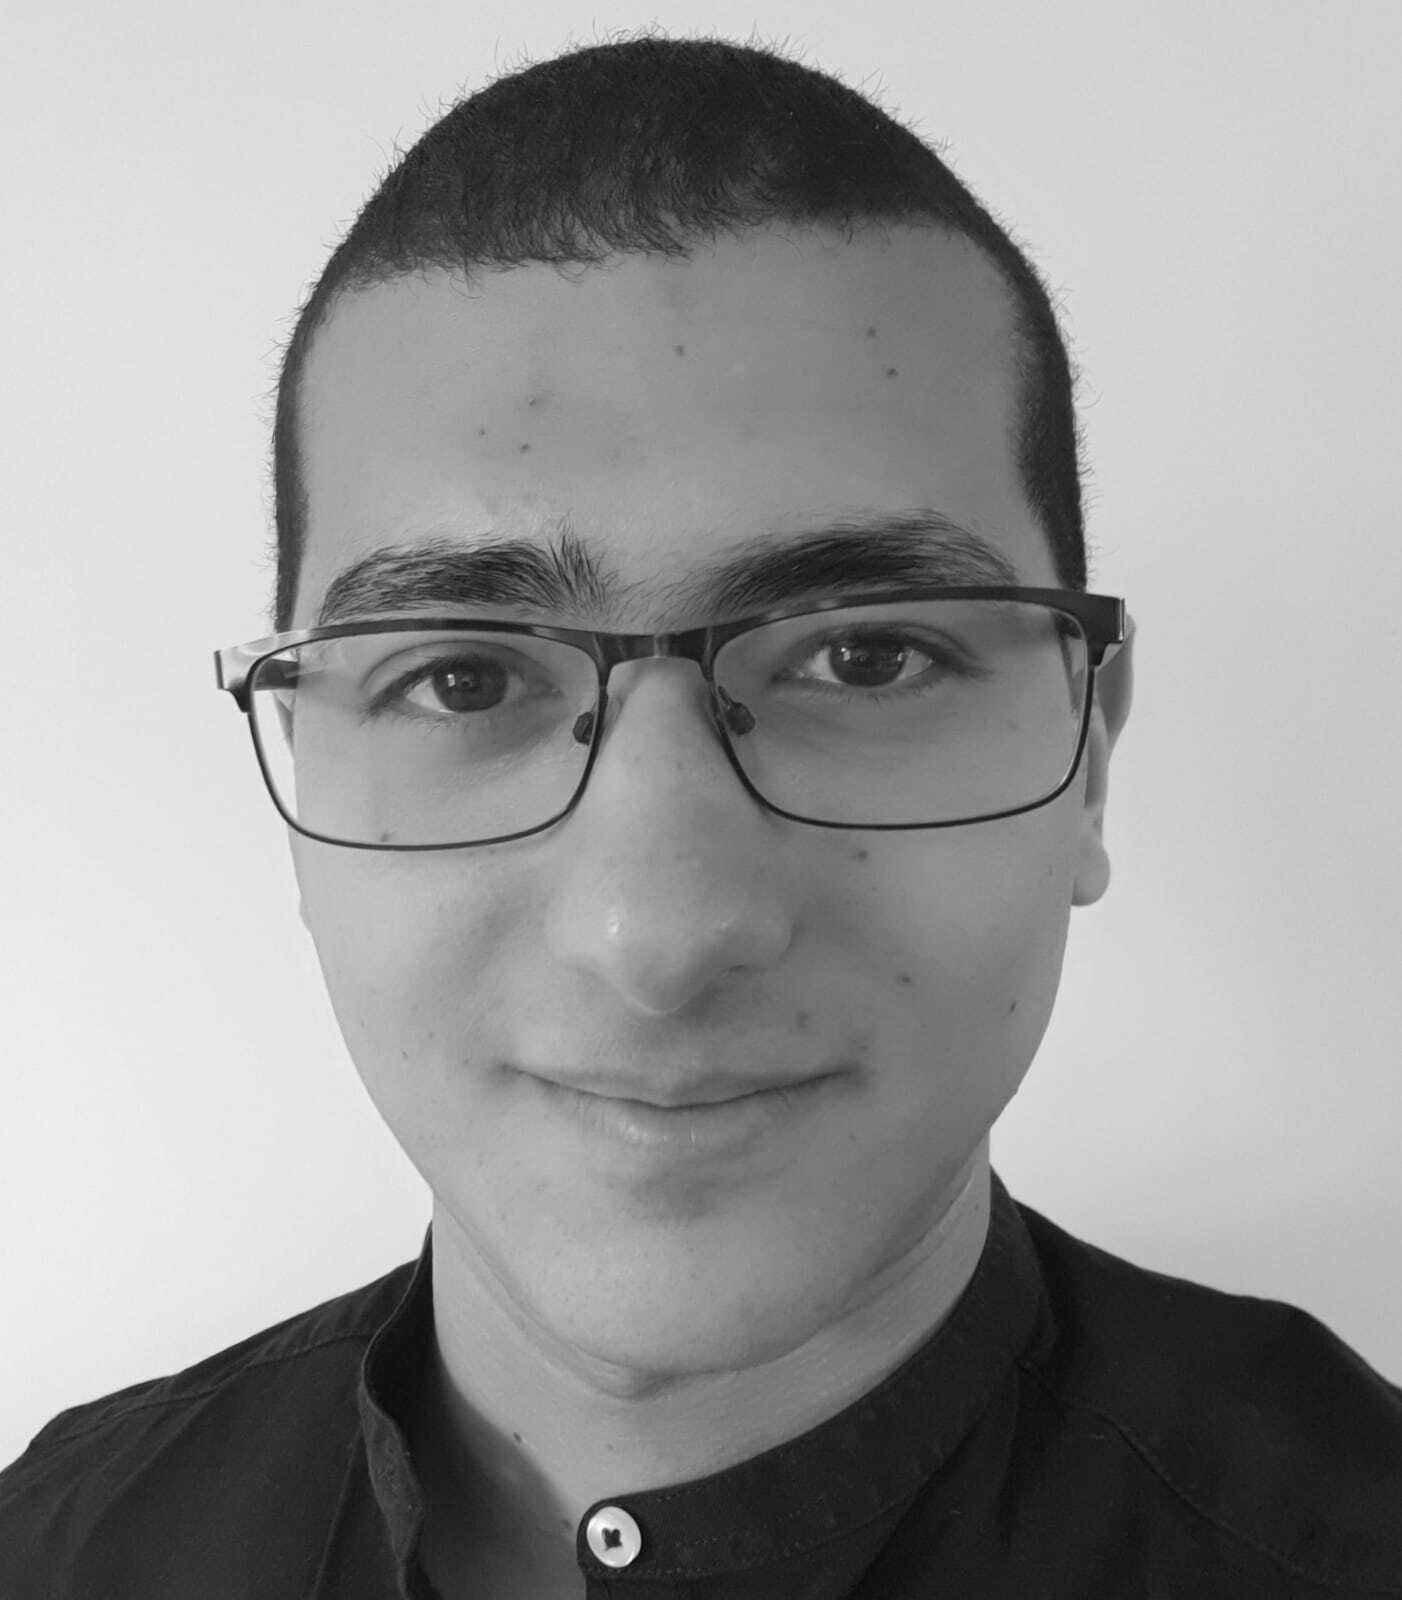
\includegraphics[width=1in,height=1.25in,clip,keepaspectratio]{other/mugs/abanoub}}]{Abanoub Ghobrial}
% received the MEng degree in mechanical engineering from the University of Bristol, Bristol,  U.K., in 2018. He is currently pursuing the Ph.D. degree in computer science at the University of Bristol and is a part-time Research Associate with the Trustworthy Systems Lab, Bristol,  U.K. From 2018 to 2020, he was a full-time Research Associate with the Trustworthy Systems Lab. His current research interests are techniques to allow self-managing of autonomous safety-critical systems via continual learning during operation; and the development of simulation-based verification techniques for autonomous systems.
% \end{IEEEbiography}


% \begin{IEEEbiography}[{\includegraphics[width=1in,height=1.25in,clip,keepaspectratio]{other/mugs/kie}}]{{Kerstin Eder}} 
% is Professor of Computer Science and heads the Trustworthy Systems Laboratory at the University of Bristol, UK. She also leads the Verification and Validation for Safety in Robots research theme at the  Bristol Robotics Laboratory. She has gained extensive experience of verifying complex microelectronic designs while working with leading semiconductor design and Electronic Design Automation companies worldwide. Her research is focused on specification, verification and analysis techniques to verify or explore a system's behaviour in terms of functional correctness, safety, security, performance and energy efficiency. Prof.\ Eder's most recent contributions include agent-based testing, how to use assertions and theorem proving to verify control system designs, energy modeling and static resource analysis techniques to predict energy consumption of software. She holds a PhD in Computational Logic and an MSc in Artificial Intelligence from the University of Bristol, UK, as well as an MEng in Informatics (Dipl.\,Inf.) from the Technical University Dresden, Germany. In 2007 she was awarded an ``Excellence in Engineering'' prize from the Royal Academy of Engineering, UK.

% \end{IEEEbiography}


% ***************************************************
%  Appendix
% ***************************************************

\end{document}
